\documentclass[10pt,letterpaper]{article}
\usepackage[top=0.85in,left=2.75in,footskip=0.75in]{geometry}

% amsmath and amssymb packages, useful for mathematical formulas and symbols
\usepackage{amsmath,amssymb}

% Use adjustwidth environment to exceed column width (see example table in text)
\usepackage{changepage}

% Use Unicode characters when possible
\usepackage[utf8x]{inputenc}

% textcomp package and marvosym package for additional characters
\usepackage{textcomp,marvosym}

% cite package, to clean up citations in the main text. Do not remove.
\usepackage{cite}

% Use nameref to cite supporting information files (see Supporting Information section for more info)
\usepackage{nameref,hyperref}

% line numbers
\usepackage[right]{lineno}

% ligatures disabled
\usepackage{microtype}
\DisableLigatures[f]{encoding = *, family = * }

% color can be used to apply background shading to table cells only
\usepackage[table]{xcolor}

% array package and thick rules for tables
\usepackage{array}

% create "+" rule type for thick vertical lines
\newcolumntype{+}{!{\vrule width 2pt}}

% create \thickcline for thick horizontal lines of variable length
\newlength\savedwidth
\newcommand\thickcline[1]{%
  \noalign{\global\savedwidth\arrayrulewidth\global\arrayrulewidth 2pt}%
  \cline{#1}%
  \noalign{\vskip\arrayrulewidth}%
  \noalign{\global\arrayrulewidth\savedwidth}%
}

% \thickhline command for thick horizontal lines that span the table
\newcommand\thickhline{\noalign{\global\savedwidth\arrayrulewidth\global\arrayrulewidth 2pt}%
\hline
\noalign{\global\arrayrulewidth\savedwidth}}


% Remove comment for double spacing
\usepackage{setspace} 
\doublespacing

% Text layout
\raggedright
\setlength{\parindent}{0.5cm}
\textwidth 5.25in 
\textheight 8.75in

% Bold the 'Fig #' in the caption and separate it from the title/caption with a period
% Captions will be left justified
\usepackage[aboveskip=1pt,labelfont=bf,labelsep=period,justification=raggedright,singlelinecheck=off]{caption}
\renewcommand{\figurename}{Fig}

% Use the PLoS provided BiBTeX style
\bibliographystyle{plos2015}

% Remove brackets from numbering in List of References
\makeatletter
\renewcommand{\@biblabel}[1]{\quad#1.}
\makeatother

% Leave date blank
\date{}

% Header and Footer with logo
\usepackage{lastpage,fancyhdr,graphicx}
\usepackage{epstopdf}
\pagestyle{myheadings}
\pagestyle{fancy}
\fancyhf{}
\setlength{\headheight}{27.023pt}
\lhead{
\includegraphics[width=2.0in]{PLOS-submission.eps}}
\rfoot{\thepage/\pageref{LastPage}}
\renewcommand{\footrule}{\hrule height 2pt \vspace{2mm}}
\fancyheadoffset[L]{2.25in}
\fancyfootoffset[L]{2.25in}
\lfoot{\sf PLOS}

%% Include all macros below

\newcommand{\lorem}{{\bf LOREM}}
\newcommand{\ipsum}{{\bf IPSUM}}

%% END MACROS SECTION


\begin{document}
\vspace*{0.2in}

% Title must be 250 characters or less.
\begin{flushleft}
{\Large
\textbf\newline{Multi-Domain Finite Element Meshing for Parotid Acinar Cell Modeling and Simulation}
% Please use "sentence case" for title and headings (capitalize only the first word in a title (or heading), the first word in a subtitle (or subheading), and any proper nouns).
}
\newline
% Insert author names, affiliations and corresponding author email (do not include titles, positions, or degrees).
\\
John Rugis\textsuperscript{1*},
Nathan Pages\textsuperscript{1},
David Yule\textsuperscript{2},
James Sneyd\textsuperscript{1}
\\
\bigskip
\textbf{1} Department of Mathematics,University of Auckland, Auckland, New Zealand
\\
\textbf{2} School of Medicine and Dentistry, University of Rochester, Rochester, NY, USA
\\

\bigskip

% Insert additional author notes using the symbols described below. Insert symbol callouts after author names as necessary.
% 
% Remove or comment out the author notes below if they aren't used.
%
% Primary Equal Contribution Note
%\Yinyang These authors contributed equally to this work.

% Additional Equal Contribution Note
% Also use this double-dagger symbol for special authorship notes, such as senior authorship.
%\ddag These authors also contributed equally to this work.

% Current address notes
%\textcurrency Current Address: Dept/Program/Center, Institution Name, City, State, Country % change symbol to "\textcurrency a" if more than one current address note
%% \textcurrency b Insert second current address 
%% \textcurrency c Insert third current address

% Use the asterisk to denote corresponding authorship and provide email address in note below.
* j.rugis@auckland.ac.nz
\end{flushleft}

% Please keep the abstract below 300 words
\section*{Abstract}
Full 3-D structural reconstruction of biological cells is necessary for modeling and simulation used to explore,
among other things, the effects of physically accurate spatial heterogeneities. Such reconstructions usually
take the form of surface and volumetric meshes which can be used for both visualisation and numerical
simulation. We report a method for constructing multi-domain finite element meshes that we used to model
calcium dynamics in parotid acinar cells. Parotid acinar cells interact with each other across physically close
interfaces that need to be retained in the meshes. Our meshes are derived from microscopy image stacks of
real cells and as such are physically accurate. We employ an iterative coupled mesh refinement process to
generate and maintain common conformal faces between adjacent cells. Termination of the refinement
process is guided by a reference target surface curvature characteristic for each cell. Test simulations were
run to verify the quality of the generated meshes.\\

\section*{Introduction}
The primary role of salivary gland acinar cells is to secrete saliva, the lack of which causes a host of severe medical difficulties \cite{fox1985,melvin1991}. Thus, an understanding of the mechanisms underlying saliva secretion are vital for the understanding of oral health.  The basic mechanism of saliva secretion is well understood \cite{nauntofte1992}, and has been previously modeled in detail.
In brief, agonist stimulation (by hormones or neurotransmitters) leads to the production of the second messenger, inositol trisphosphate (IP\textsubscript{3}), which then releases Ca\textsuperscript{2+} from the endoplasmic reticulum (ER) through IP\textsubscript{3} receptors (IPR) which are also Ca\textsuperscript{2+} channels. Ca\textsuperscript{2+} released from the ER is then pumped back into the ER by Ca\textsuperscript{2+} ATPase pumps (SERCA) or removed from the cell by plasma membrane ATPases.\\

Feedback between Ca\textsuperscript{2+} and IPR, as well as between Ca\textsuperscript{2+} and IP\textsubscript{3} production and degradation, leads to repetitive cycles of Ca\textsuperscript{2+} release and reuptake, and thus to periodic Ca\textsuperscript{2+} spikes. Stochastic properties of the IPR are also closely involved in determining the interspike interval.
These Ca\textsuperscript{2+} spikes activate Cl\textsuperscript{-} channels (in the apical region of the acinar cell) and K$^+$ channels (in the basal region of the cell), leading to flow of Cl\textsuperscript{-} and K\textsuperscript{+} out of the cell, but in different directions. These ionic flows, in turn, set up ionic gradients that drive the flow of water through the cell, via osmosis.\\

A critical feature of salivary gland acinar cells is their spatial organisation \cite{Sneyd2017383}. The apical and basal regions of the cell have different sets of ion channels, and open into different environments. These spatial heterogeneities are the reason that salivary acinar cells can transport water (i.e., produce saliva) in a specified direction.
Although much is understood about saliva secretion, important questions, both experimental and theoretical, remain. From the theoretical point of view, one of the most interesting questions is how the structure of the acinar cells affects the properties of the Ca\textsuperscript{2+} spikes. IPR are not distributed uniformly through the cell, but are concentrated in the apical region. Furthermore, IP\textsubscript{3} is produced only at the basal membrane. There is thus a significant spatial separation between the various components of the feedback system that governs oscillatory Ca\textsuperscript{2+} spiking. How these spatial heterogeneities might affect Ca\textsuperscript{2+} dynamics is one of the most important current theoretical questions in the study of how Ca\textsuperscript{2+} spiking controls saliva secretion.\\

We have previously studied the effects of spatial heterogeneity in a single parotid acinar cell, with a structure that is determined from experimental measurements \cite{sneyd2003}. However, acinar cells do not sit in isolation. Each cell is situated in group, called an acinus, that resembles a bunch of grapes. Inside each acinus, each parotid cell is coupled to neighbouring acinar cells by gap junctions, and all secrete water into a common lumen that has a highly branched structure. This means that the properties of the Ca\textsuperscript{2+} spikes cannot be properly determined by the consideration of an isolated cell. Furthermore, the rate at which an acinus secretes water (into a common lumen) may be influenced by the structure of the lumen, which determines the network structure of the acinus, as well as which cells lie `downstream' of other cells.\\

For a proper understanding of saliva secretion, and how it is affected by spatial heterogeneities, all these complications must be taken into account. Thus, here we extend our initial single-cell model to a multicellular model of an acinus of seven cells (the smallest acinus for which we have the detailed anatomical structure).
We focus here on the technical details of mesh construction, leaving details of the scientific results for a subsequent publication.\\

\section*{Description of Method}

Our work flow has three sequential steps:
\begin{enumerate}
\item Image segmentation
\item Surface triangulation and refinement
\item Volumetric meshing
\end{enumerate}

\subsection*{Image segmentation}

By visual inspection we identified and selected a contiguous clump of seven cells within our source data image stack.  This clump spanned thirty of the images and covered a maximum of approximately one-quarter of each image. Segmentation was done manually by tracing the outline of each cell in each image with a distinct color, followed by matched color flood-fill. One-quarter of original image number 16, along with its segmentation, is shown in Fig~\ref{fig:slice}.\\

\begin{figure}[!h]
%\begin{center}
%\fbox{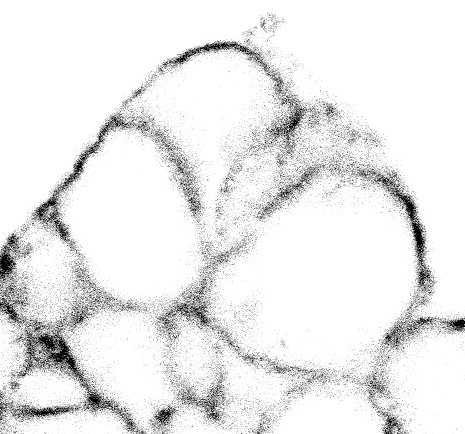
\includegraphics[width=0.45\textwidth]{images/cells-stack-16_crop.jpg}}
%\hspace{0.5cm}
%\fbox{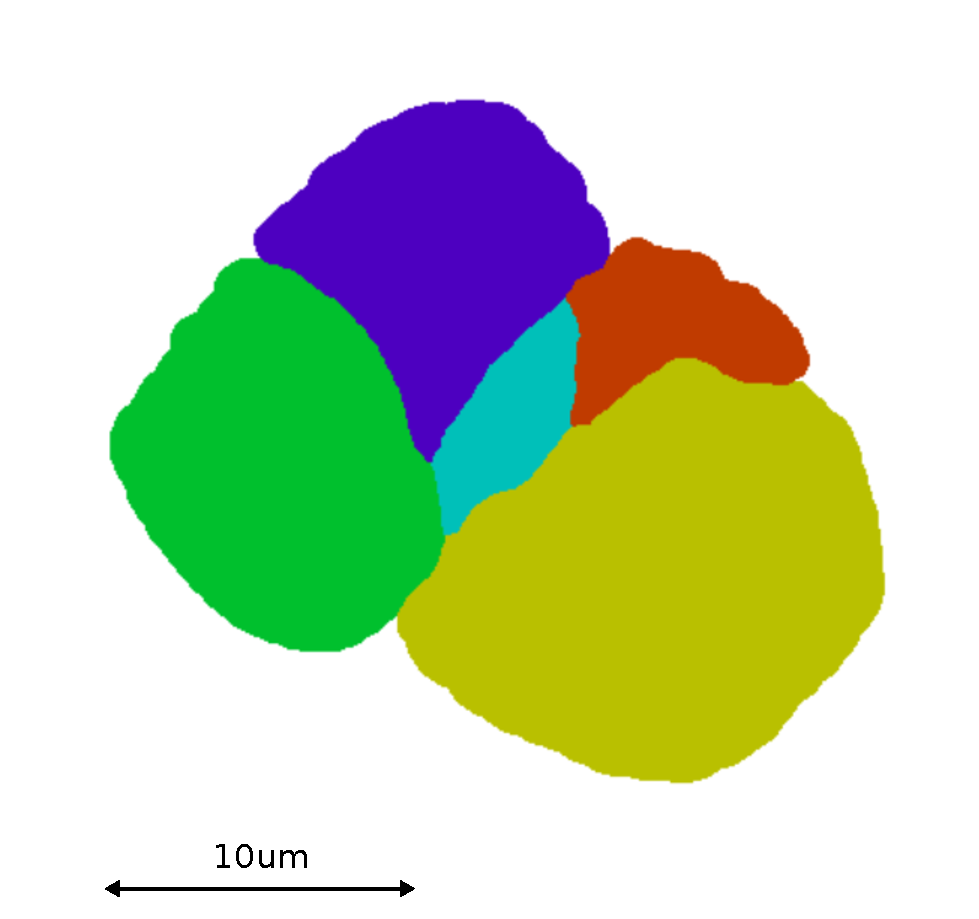
\includegraphics[width=0.45\textwidth]{images/segmented.pdf}}
%\end{center}
\caption{Subsection of a microscopy image slice on the left and its segmentation on the right.}
\label{fig:slice}
\end{figure}

Note that with our image stack the ratio of stack spacing to pixel resolution is 11.6 (being $0.069/0.80$). To bring this closer to a ratio of one-to-one, we reduced the X and Y dimensions in the segmented image stack by a factor of four using nearest neighbor interpolation (to retain the distinct coloring of each cell) resulting in a pixel spacing of approximately $0.28\mu\textrm{m}$.  The reduced images were then combined into a single XYZ TIFF stack for convenience.\\

\subsubsection*{Curvature}

We also wanted to extract some information from the segmented image stack about the smoothness of the surface of each cell. We chose line curvature as a surface smoothness characteristic indicator. Both line and surface curvature have been used successfully  by one of us (Rugis) in other work to characterize the surface of objects \cite{Rugis_2005_SCMMD, Rugis_2006_SRMRSD, Rugis_2006_SISCE}. A description of how we used characteristic line curvature information as a reference for guidance in a cell surface curvature smoothing process in this current work will be given in following sections.\\

For curvature calculation purposes, we went back to the $1024 \times 1024$ segmented images and extracted pixels associated with the closed curve boundary outline for each cell in each  image, then selected the outline containing the maximum number of pixels for each cell as being the closest to a ``great arc" slice through that cell. This great arc criterion was based on the fact that only the curvature associated with a great arc of a sphere is equal to the sphere surface mean curvature.\\

Next, considering that fact that image pixels are all located on a regular rectangular grid (not very useful for calculating actual local curvature!), a smoothed version of each cell outline was created using a 2D Savitzky-Golay (least-squares) fitting filter \cite{doi:10.1021/ac60214a047}. Fig \ref{fig:slice_outline} shows a sample cell outline with the original pixel locations as well as the smoothing process result.\\

\begin{figure}[h!]
%\begin{center}
%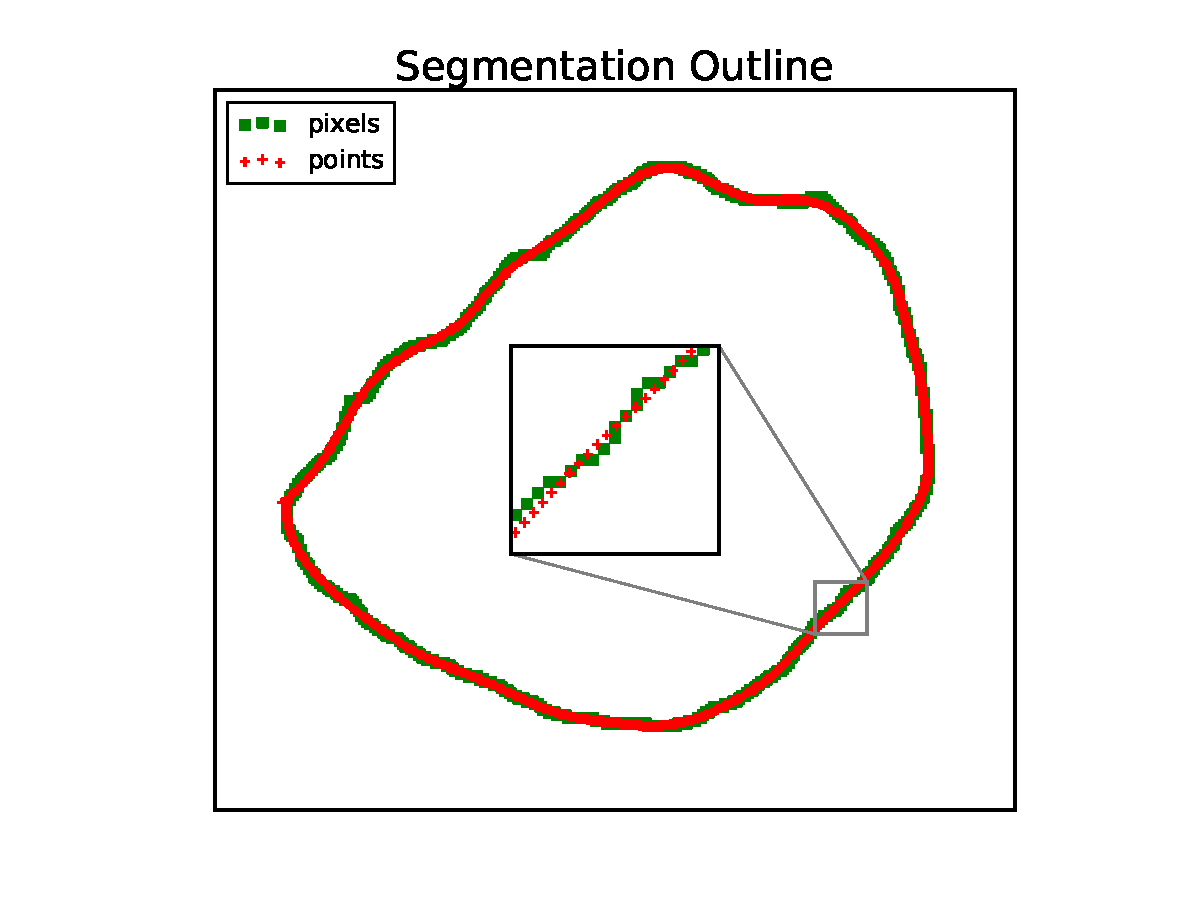
\includegraphics[width=0.5\textwidth]{images/outline.pdf}
%\end{center}
%\vspace{-5mm}
\caption{A sample segmentation pixel outline in green with smoothed node points in red.}
\label{fig:slice_outline}
\end{figure}

Planar line curvature was calculated at each point on the smoothed outlines using a local estimator as given in \cite{Rugis_2008_DSC}. We used weighted histograms to visualise the curvature distribution for each of the seven cells. Two of the histograms are shown in Fig \ref{fig:ref_histogram}. Note that in both cases the curvature distribution is biasing towards the positive, as would be expected with any closed curve from the outside using the convention that positive curvature is associated with convex line segments.\\

\begin{figure}[h!]
%\begin{center}
%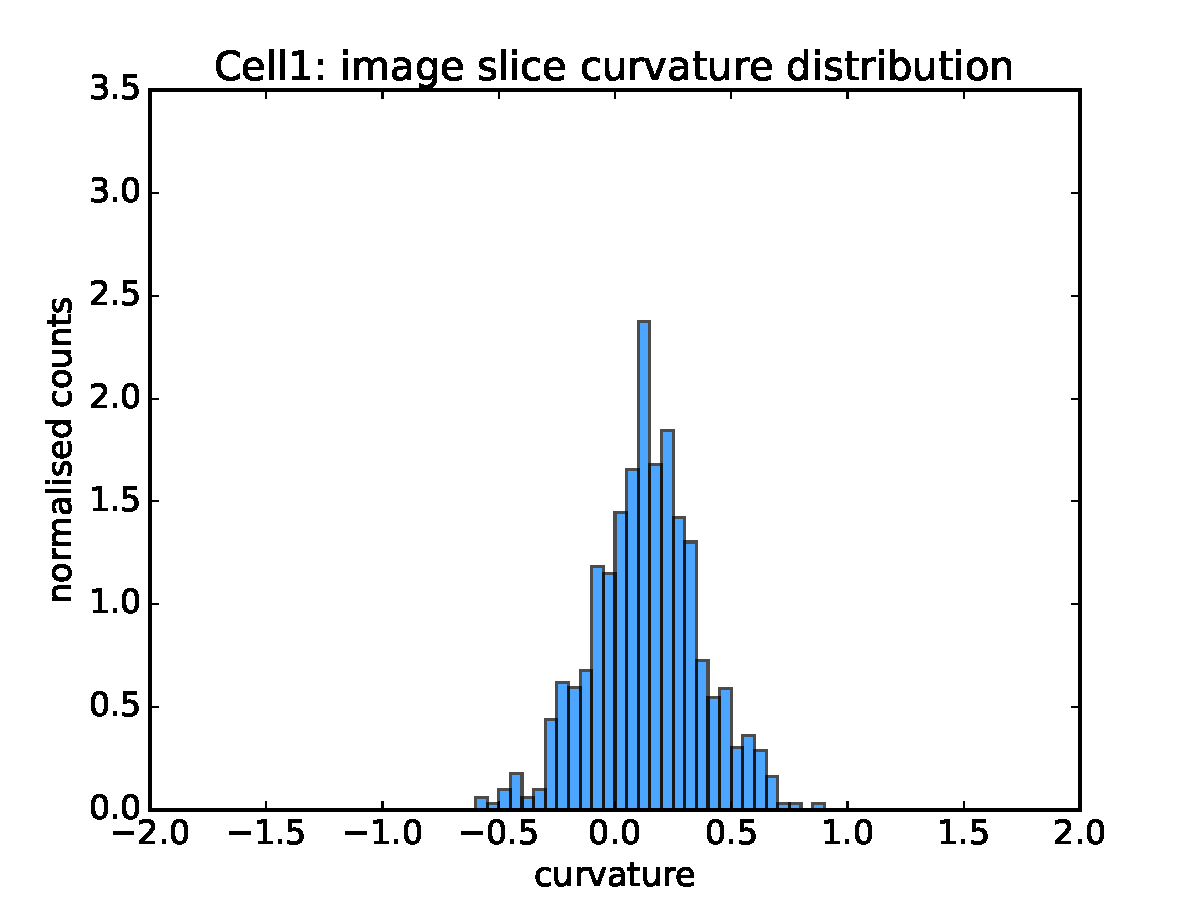
\includegraphics[width=0.4\textwidth]{images/cell1_curv.pdf}
%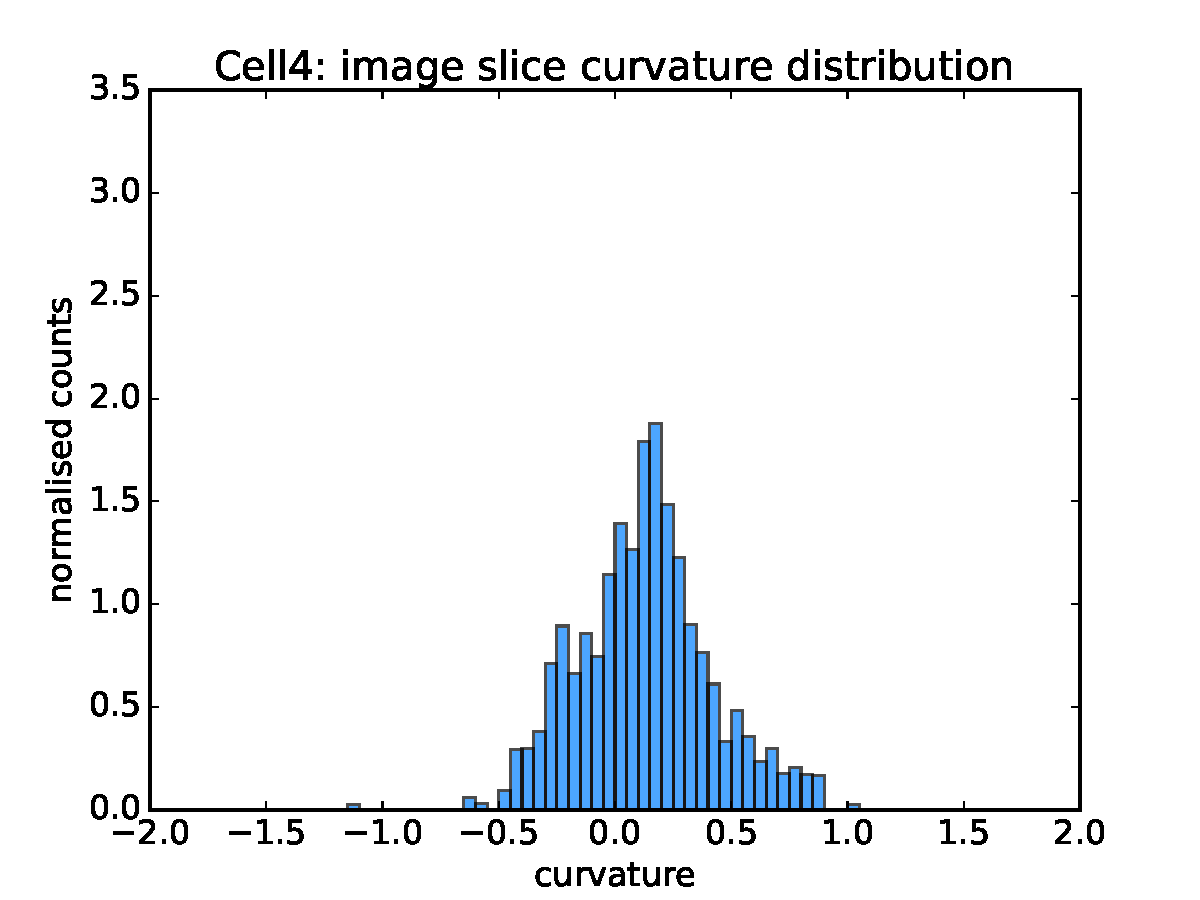
\includegraphics[width=0.4\textwidth]{images/cell4_curv.pdf}
%\end{center}
\caption{Reference curvature histograms for two of the cells (in $\mu \textrm{m}^{-1}$). The distributions are ``near normal".}
\label{fig:ref_histogram}
\end{figure}

To simplify our characterisation of cell surface shape we chose the weighted standard deviation of the curvatures for each cell as a single valued characterisation of surface smoothness and, in that sense, a signature for the shape of each cell.
This signature is indicative (i.e. not unique) because standard deviation is only an unambiguous characterisation given normally distributed data.
The weighted curvature standard deviation for each of the seven cells is shown in Table \ref{tab:ref_curv}.\\ 

\begin{table}[ht!]
\begin{center}
%\footnotesize
\begin{tabular}{|c|c|}
\hline
\rule{0pt}{3ex} cell &curvature std ($\mu \textrm{m}^{-1}$) \\
\hline
\rule{0pt}{3ex} 1 &0.2305\\
2 &0.3567\\
3 & 0.3864\\
4 &0.2832\\
5 &0.6868\\
6 &0.3627\\
7 & 0.4226\\
\hline
\end{tabular}
\end{center}
\caption{The standard deviation of curvature values for seven cells extracted from the microscopy image stack.}
\label{tab:ref_curv}
\end{table}

\subsection*{Surface triangulation and refinement}

For the surface triangulation and refinement process we started with the reduced XYZ TIFF image stack described in the previous section. We treat this reduced stack as a $256\times 256 \times 31$ solid voxel block within which each voxel is labeled with a color associated with the cell that it belongs to. 

\subsubsection*{Surface triangulation}

Significant prior work in extracting triangle surface meshes from labelled voxel blocks has been done by Boltcheva et al.\cite{boltcheva:inria-00420228} and we used their technique. Sample computer code implementing this technique was found on the Computational Geometry Algorithms Library (CGAL) web site (\url{www.cgal.org}). Note that we needed to convert our voxel block data to Inria format (\url{www.inria.fr}) before passing it to the CGAL code.

The output from the CGAL code was a multi-domain triangle surface mesh, as shown in Fig \ref{fig:rough}, where each of the cell faces are labeled in color by cell. However, there are two problems with this mesh: there are ``steps" as a result of the relatively limited stack resolution and, on close inspection, the surfaces are rather rough (as can be seen more clearly in the cell labeled ``no smoothing" in the top of Fig \ref{fig:cell_morph}). This lack of surface smoothness has the net effect of increasing the surface area of each cell to a value larger than what it most likely is in the real cells.\\

\begin{figure}[h!]
%\begin{center}
%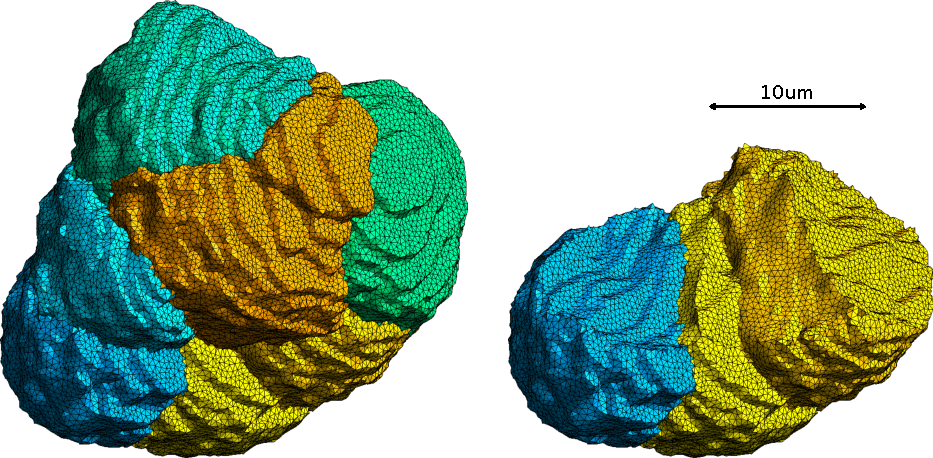
\includegraphics[width=0.8\textwidth]{images/rough.pdf}
%\end{center}
\caption{Rough multi-domain surface mesh: all seven cells (left) and three exposed cells (right).}
\label{fig:rough}
\end{figure}

\begin{figure}[h!]
%no smoothing 
%\includegraphics[width=0.2\textwidth]{images/cell1-C0_crop.png}
%\begin{center}
%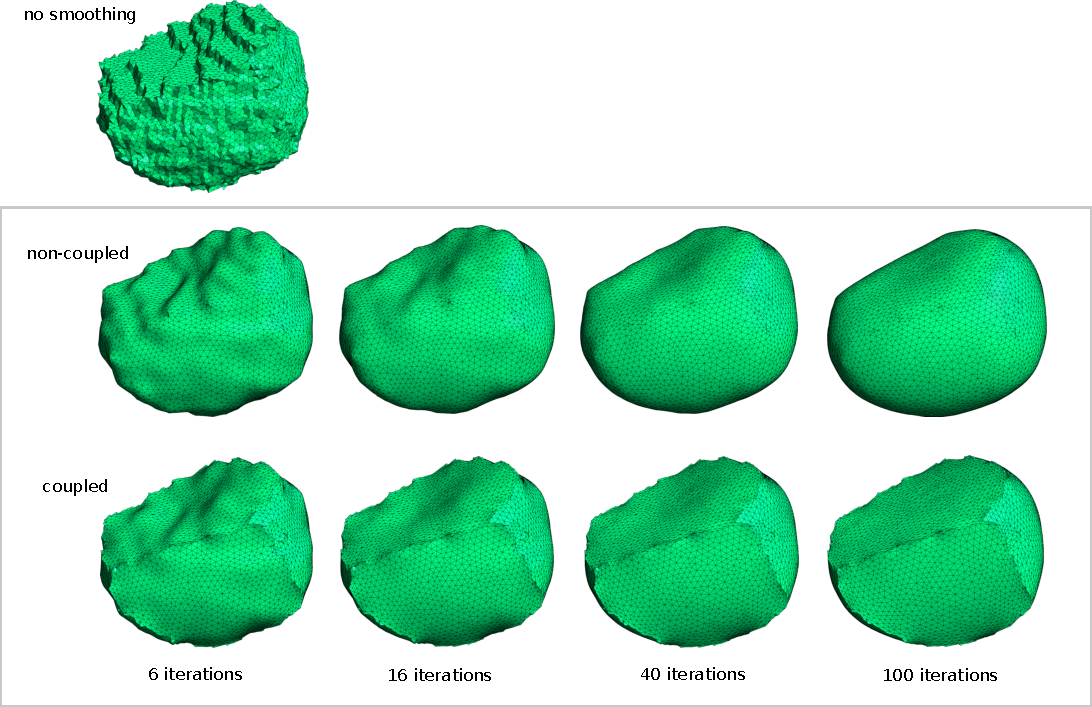
\includegraphics[width=0.9\textwidth]{images/evolution.pdf}
%\end{center}
\caption{Cell smoothing evolution, with and without inter-cell coupling.}
\label{fig:cell_morph}
\end{figure}

\subsubsection*{Surface smoothing}

To reduce the surface area closer to what it should be, we created a constrained surface smoothing process. Note that the smoothing process should: 1) minimise the surface area of each cell while 2) maintain the volume of each cell and 3) keep the shared conformal faces between cells as being shared.\\

A pseudo-code outline for our iterative smoothing process is as follows:
\begin{verbatim}
Main Loop
{
    Cell Loop (for each cell)
    {
        Smooth the cell.
        Restore volume of cell.
        Calculate the cell surface curvature.
    }
    Have all cells reached the target curvature?
        Yes: DONE, exit loop.
        No: Go back to top of Main Loop.  
}
\end{verbatim}

For each cell we used the curvature-flow based smoothing operation described in \cite{Desbrun:1999:IFI:311535.311576}. Note that the cell smoothing process works by slightly moving the position of the surface mesh vertices for each cell in turn (with no new faces added or any faces removed). Therefore, vertices associated with shared faces get moved twice in each pass through the Main Loop, i.e. once for each cell in every adjacent pair of cells. In this sense, the smoothing is a coupled process. With our approach, if the vertices associated with shared faces were allowed to split from each other, the result would be non-coupled as shown in the middle row of Fig \ref{fig:cell_morph}, which is not what is required.\\

Coupled smoothing results after each of each of 6, 16, 40 and 100 iterations are shown in the bottom row of Fig \ref{fig:cell_morph}.
The question remains: after how many iterations should we stop? This is where we found the weighted curvature standard deviation values from Table \ref{tab:ref_curv} useful as will be described in the next section.\\

\subsubsection*{Iteration termination}

Recall from the previous section that reducing cell surface area while at the same time maintaining cell volume was an important consideration. The smoothing step in our process has the effect of reducing surface area as shown for one hundred iterations in the left-hand side of Fig \ref{fig:100_iterations}. The greatest rate of surface area reduction occurs within the first ten iterations or so. Cell volume is explicitly restored in our process, and thus remains almost unchanged, as can be seen in the right-hand side of Fig \ref{fig:100_iterations}. (The raw data for these plots are given in Appendix Tables \ref{tab:surf} and \ref{tab:vol}.) For further guidance as to when to terminate the iterative process we looked to surface curvature.\\

\begin{figure}[h!]
%\begin{center}
%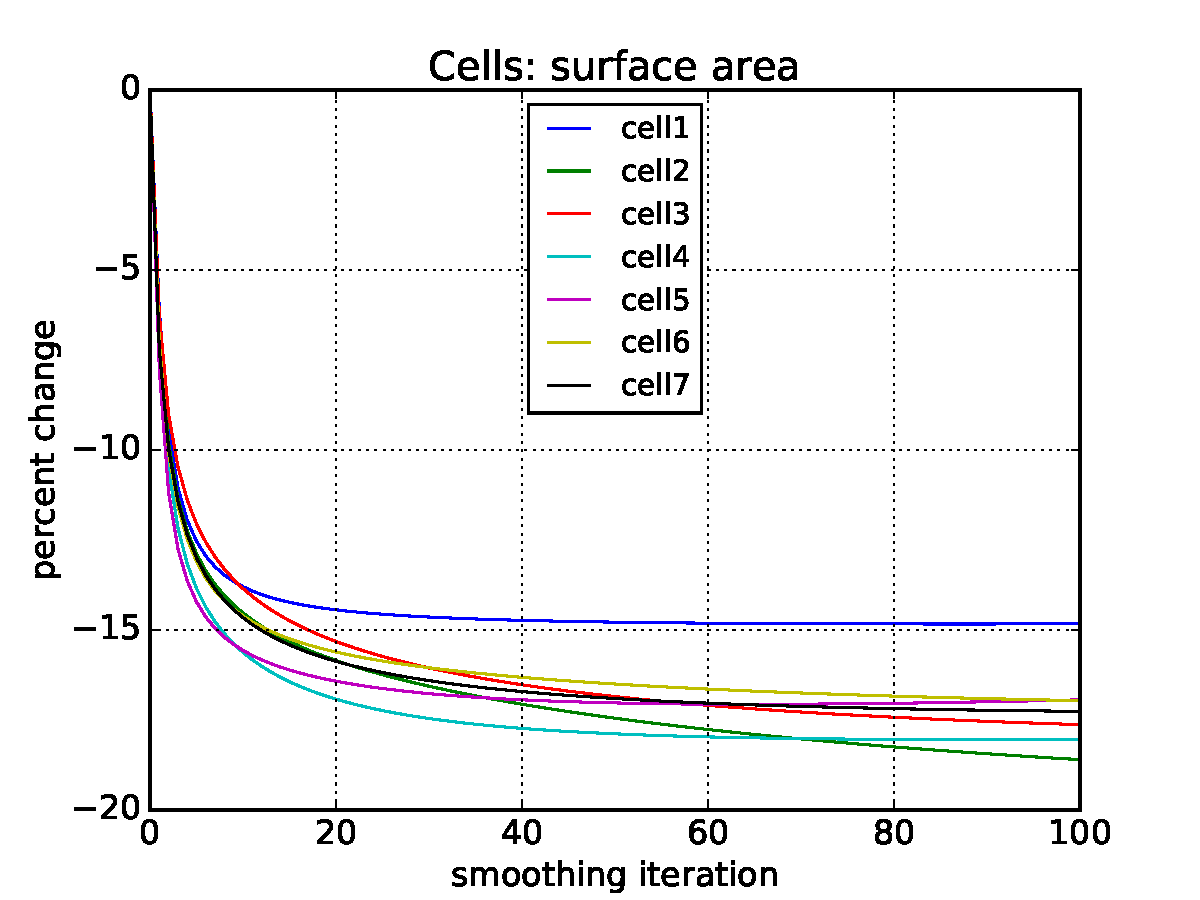
\includegraphics[width=0.45\textwidth]{images/cell_surf_100.pdf}
%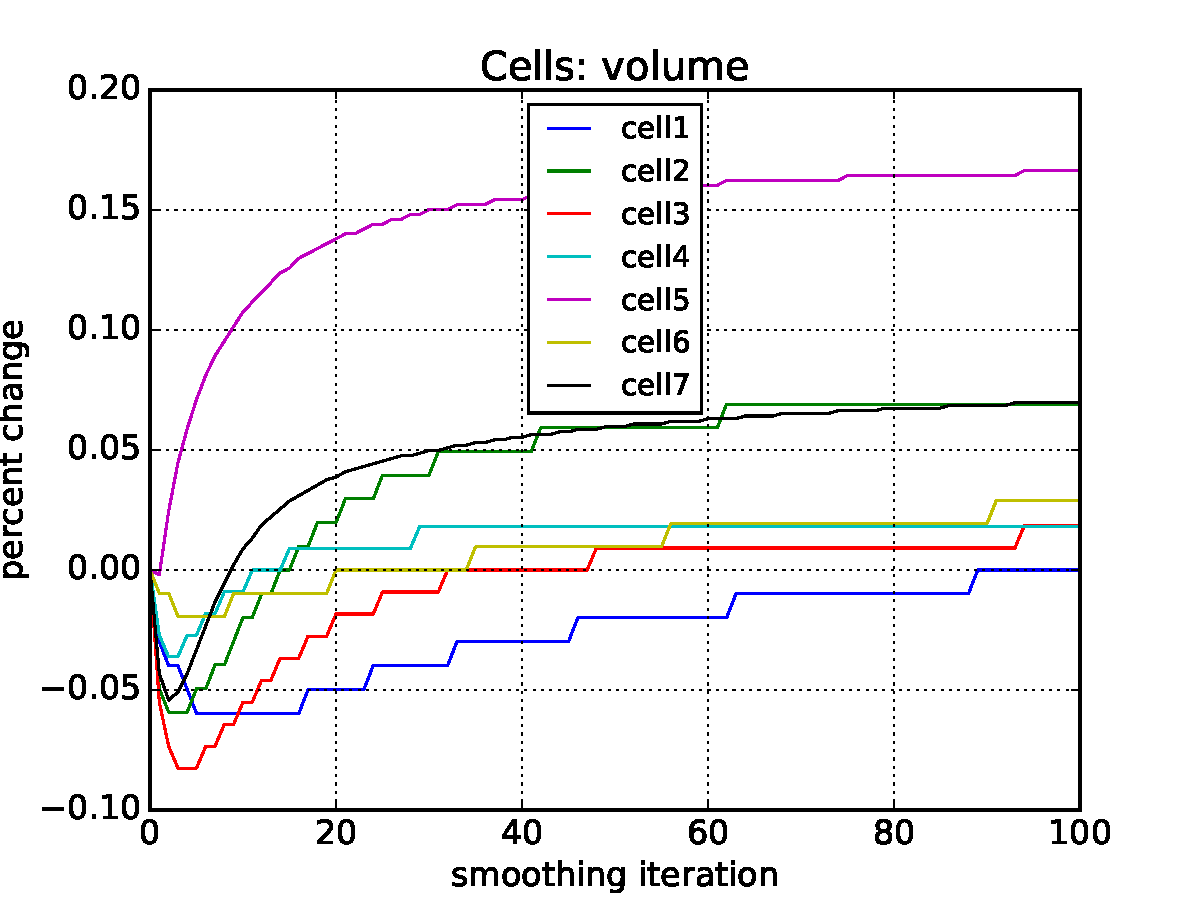
\includegraphics[width=0.45\textwidth]{images/cell_vol_100.pdf}
%\end{center}
\caption{Cell surface area and volume evolution over one hundred coupled smoothing iterations. (Note the much smaller scale range with the plot on the right.)}
\label{fig:100_iterations}
\end{figure}

For each cell, in every iteration, we calculated the 2D surface curvature at every mesh vertex using the (local) surface curvature estimator given in \cite{Rugis_2008_DSC}. And for each cell, in every iteration, we calculated the weighted standard deviation of those curvatures to get a single smoothness characteristic value. We then compared this value to the associated target standard deviation in Table \ref{tab:ref_curv} and expressed it as a ratio as shown in Fig \ref{fig:curv_std}. The raw data for this plot is given in Appendix Table \ref{tab:curv}.\\

\begin{figure}[h!]
%\begin{center}
%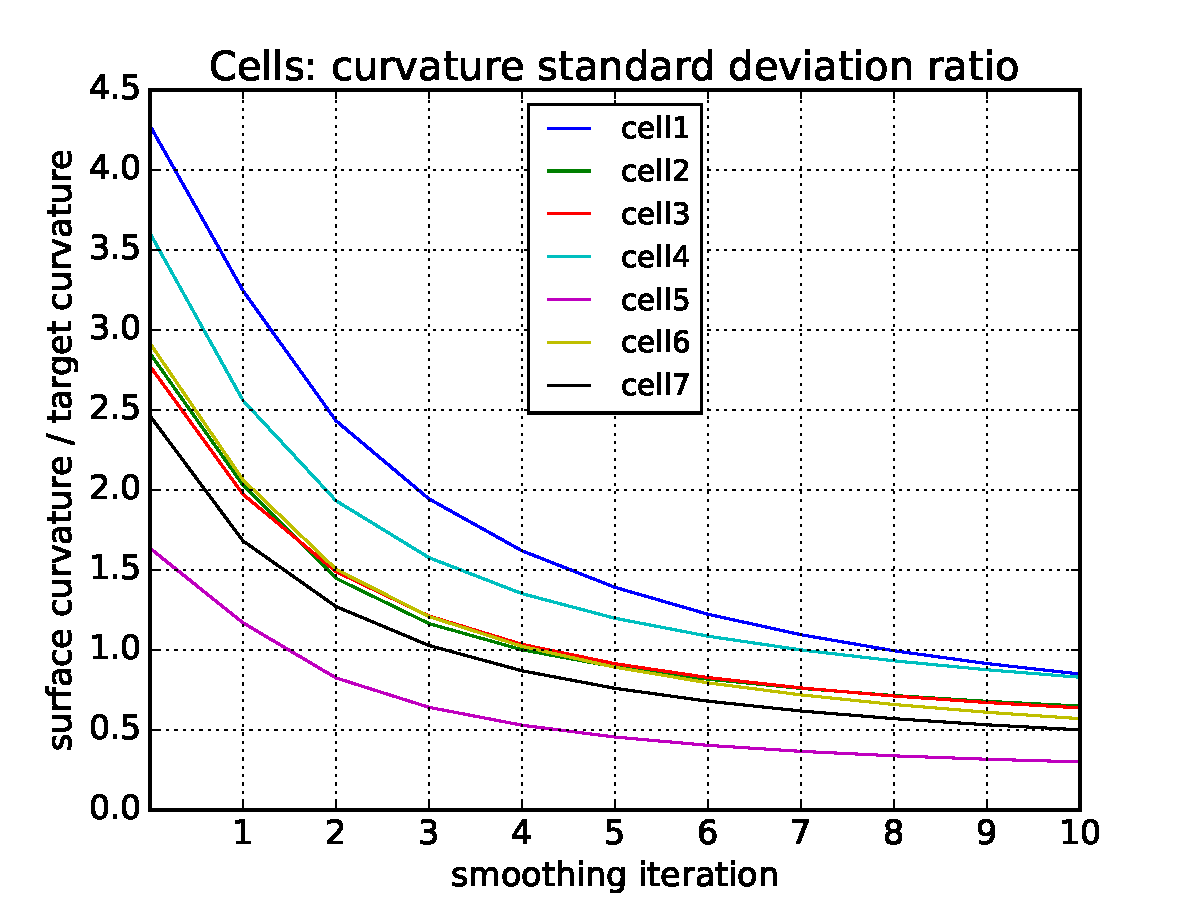
\includegraphics[width=0.45\textwidth]{images/cell_curv_std.pdf}
%\end{center}
\caption{All of the cells hit the target curvature standard deviation ratio of one after nine iterations.}
\label{fig:curv_std}
\end{figure}

With this information in hand, we decided to terminate the iterative process and accept the results after ten iterations by which time all of the cells had more than dropped below their target characteristic curvature.\\

For further insight and confirmation of our results we produced initial and final iteration weighted surface curvature histograms for each of the seven cells. Histograms for two of the cells are shown in Fig \ref{fig:morph_histogram}. Note that in all cases, as expected, the initial curvature spread was relatively wide and the final curvature distribution narrower, peaking just to the right (positive) side of zero. The final curvature histograms compared favourably to those associated with the image stacks including those shown earlier in Fig \ref{fig:ref_histogram}.\\

\begin{figure}[h!]
%\begin{center}
%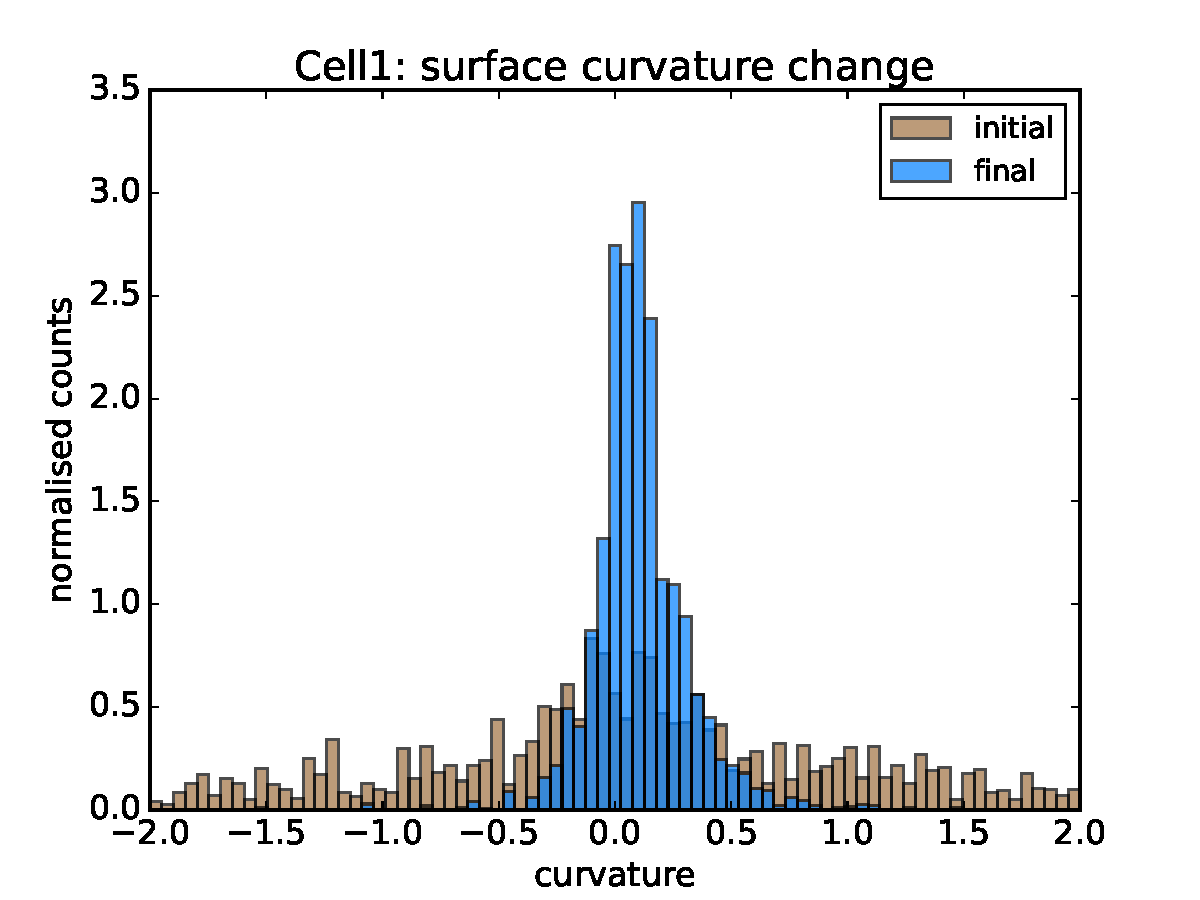
\includegraphics[width=0.4\textwidth]{images/cell1_curv_morph.pdf}
%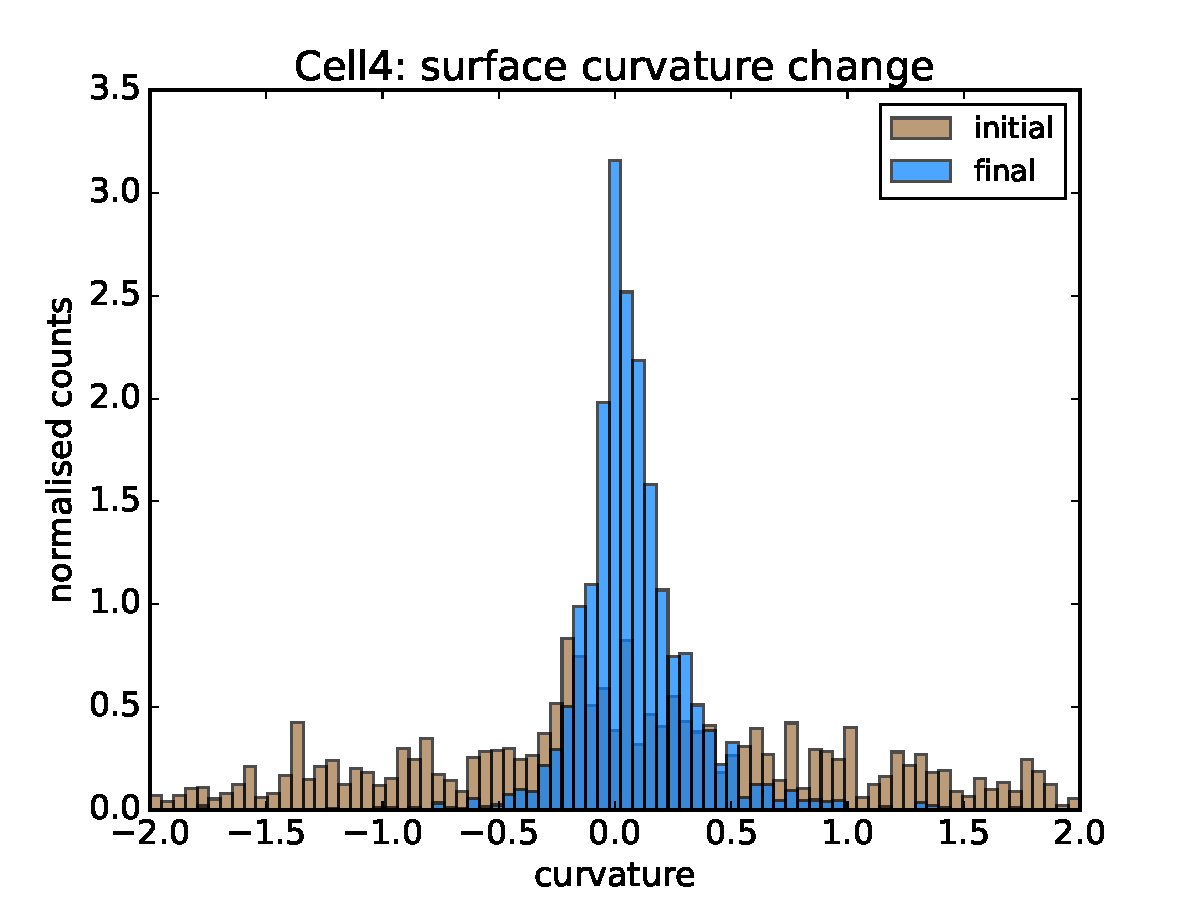
\includegraphics[width=0.4\textwidth]{images/cell4_curv_morph.pdf}
%\end{center}
\caption{Initial surface curvature distribution in brown and smoothed surface curvature in blue.}
\label{fig:morph_histogram}
\end{figure}

\subsection*{Volumetric meshing}

In the final step of our process, we filled in the surface mesh for each cell with tetrahedrons using the Gmsh software tool \cite{NME:NME2579}. This volumetric meshing employed a 3-D Delaunay refinement algorithm that reduces the instance of tetrahedral slivers, making the tetrahedrons more equilateral, thereby improving the mesh quality from the point of view of the finite element method. Note that the volumetric meshing did not alter the associated surface meshes, insuring that the meshes remained conformal. Fully meshed cells are shown in Fig \ref{fig:smooth}.\\

\begin{figure}[h!]
%\begin{center}
%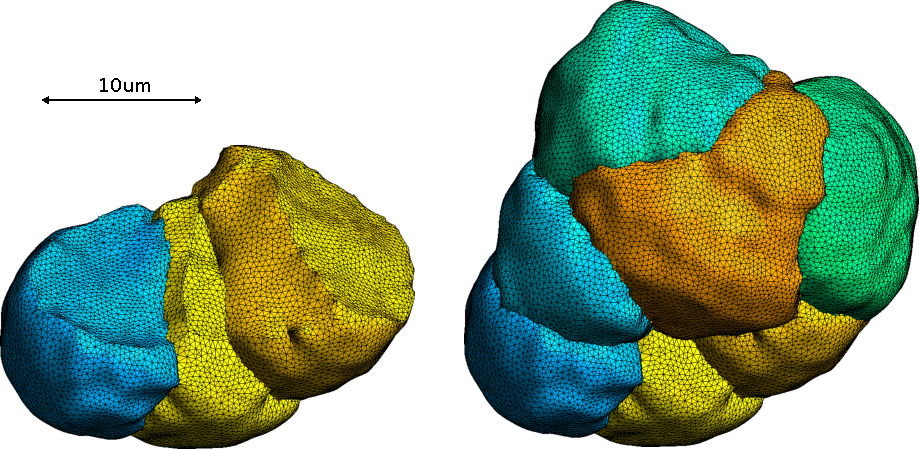
\includegraphics[width=0.8\textwidth]{images/smooth.pdf}
%\end{center}
\caption{Fully meshed smoothed cells: three exposed cells (left) and all seven cells (right).}
\label{fig:smooth}
\end{figure}

\section*{Test Simulations}
In this paper we focus on showing that our model equations can be solved on the new multicellular mesh, and that the results are consistent with previous work \cite{Sneyd2017383}, rather than focussing on the many types of responses exhibited by coupled oscillating cells.\\

We tested the meshes by using them to compute Ca\textsuperscript{2+} responses in two cells that are coupled by the diffusion of Ca\textsuperscript{2+} and IP\textsubscript{3} through gap junctions. Intercellular coupling was assumed to occur homogeneously on the entire intercellular boundary, with the intercellular flux assumed to be linearly proportional to the local concentration difference.
Importantly, our numerical scheme  conserves the total amount of calcium available, even though some calcium is exchanged between the cells. After 150s of stimulated Ca\textsuperscript{2+} oscillations, the relative amount of calcium lost (summed over both cells) is $4\times10^{-13} \mu\mathrm{M}$.\\

The cell meshes contain between 7,000 and 15,000 node points. The average distance between the nodes of the tetrahedron in the meshes is $0.46 \mu\mathrm{m}$. Any structure larger than that can be resolved with this mesh. However, this resolution is sufficient for our purposes. Firstly, our computed solutions are smoothly varying over the cell, with no sharp spatial gradients (on a length scale of less than $0.46 \mu\mathrm{m}$). Secondly, although the cells are spatially heterogeneous with clearly defined apical and basal regions, each of which has different sub-models that govern the local Ca\textsuperscript{2+} dynamics, both the apical and basal regions are large enough to be well modeled by a mesh of this spatial resolution.​\\

In the absence of intercellular coupling, the Ca\textsuperscript{2+} oscillations in each cell are identical to those obtained in uncoupled cells. However, when the cells are coupled as described above, the oscillation in one cell can have a significant effect on the response of the neighboring cell, even to the extent that oscillations can be eliminated by the coupling (results not shown). Again, these results are consistent with results obtained by solving a system of coupled ordinary differential equations, i.e., a model that ignores all spatial aspects.\\

Because of this consistency with previous work, we conclude that our multicellular conformal mesh is sufficient for the computation of multicellular coupled responses.
As an indication of the quality of our results, Fig \ref{fig:two_cells} shows a calcium concentration spike propagating from the apical region (bottom centre of the image) to the basal region (top and left) in two adjacent cells.\\ 

\begin{figure}[h!]
%\begin{center}
%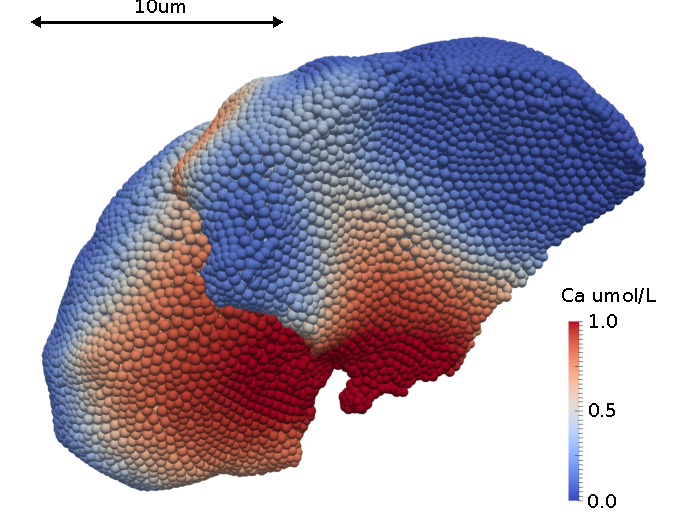
\includegraphics[width=0.58\textwidth]{images/2cells_crop.pdf}
%\end{center}
\caption{Simulation sanpshot of two interacting adjacent cells.}
\label{fig:two_cells}
\end{figure}

\section*{Discussion}

Overall the challenge in this latest work could be described as generating a physically accurate mesh model given incomplete data. As described in the section on image segmentation, the spacing between source images was relatively large compared to the source image pixel resolution.\\

The mesh design was guided by, and constrained by, both the practical requirements of finite element modeling and the simplification assumptions made in our mathematical model. We believe that our smoothing process produced meshes that are arguably organic in appearance.\\ 

There is a fine point not discussed earlier regarding how we calculated surface curvature in section on iteration termination. We decided to leave out the curvatures at points along the seams around common faces. These seams are relatively sharp as can be seen in the bottom row of Fig \ref{fig:cell_morph}. The sharp seams gave unrealistically high curvature values. In the real cells these seams are probably not so sharp as can be inferred from the left hand side image in Fig \ref{fig:slice}.\\

In our application, we believe that there is no objective collection of criteria with which to optimally decide precisely when to terminate the iterative smoothing process. However, we do believe using nominally ten iterations is well justified as described earlier in this paper.\\

\section*{Supporting information}

\paragraph*{S1 Dataset.}
\label{S1_Table}
{\bf Iteration evolution result data.}

\paragraph*{S2 Supporting Information.}
\label{S2_Supporting_Information}
{\bf Software tools.}




\section*{Acknowledgements}
This work was supported by the National Institutes of Health grant number 5R01DE019245 and by the Marsden Fund of the Royal Society of New Zealand. High-performance computing facilities and support were provided by the New Zealand eScience Infrastructure (NeSI) funded jointly by NeSI's collaborator institutions and through the Ministry of Business, Innovation and Employment's Research Infrastructure programme. Thanks to NVIDIA Corporation for a K40 GPU grant.\\

%\bibliography{references}

\begin{thebibliography}{10}

\bibitem{fox1985}
Fox PC, van~der Ven PF, Sonies BC, Weiffenbach JM, Baum BJ.
\newblock Xerostomia: evaluation of a symptom with increasing significance.
\newblock J Am Dent Assoc. 1985;110(4):519--25.

\bibitem{melvin1991}
Melvin JE.
\newblock Saliva and dental diseases.
\newblock Curr Opin Dent. 1991;1(6):795--801.

\bibitem{nauntofte1992}
Nauntofte B.
\newblock Regulation of electrolyte and fluid secretion in salivary acinar
  cells.
\newblock Am J Physiol. 1992;263(6 Pt 1):G823--37.

\bibitem{Sneyd2017383}
Sneyd J, Means S, Zhu D, Rugis J, Won JH, Yule DI.
\newblock Modeling calcium waves in an anatomically accurate three-dimensional
  parotid acinar cell.
\newblock Journal of Theoretical Biology. 2017;419:383 -- 393.
\newblock doi:{https://doi.org/10.1016/j.jtbi.2016.04.030}.

\bibitem{sneyd2003}
Sneyd J, Tsaneva-Atanasova K, Bruce JIE, Straub SV, Giovannucci DR, Yule DI.
\newblock A model of calcium waves in pancreatic and parotid acinar cells.
\newblock Biophys J. 2003;85(3):1392--405.
\newblock doi:{10.1016/S0006-3495(03)74572-X}.

\bibitem{Rugis_2005_SCMMD}
Rugis J.
\newblock Surface Curvature Maps and {M}ichelangelo's {D}avid.
\newblock In: Image and Vision Computing New Zealand 2005; 2005. p. 218--222.

\bibitem{Rugis_2006_SRMRSD}
Rugis J, Klette R.
\newblock Surface Registration Markers from Range Scan Data.
\newblock In: LNCS: Combinatorial Image Analysis. vol. 4040/2006. Berlin /
  Heidelberg: Springer; 2006. p. 430--444.

\bibitem{Rugis_2006_SISCE}
Rugis J, Klette R.
\newblock A Scale Invariant Surface Curvature Estimator.
\newblock In: LNCS: Advances in Image and Video Technology. vol. 4319/2006.
  Berlin / Heidelberg: Springer; 2006. p. 138--147.

\bibitem{doi:10.1021/ac60214a047}
Savitzky A, Golay MJE.
\newblock Smoothing and Differentiation of Data by Simplified Least Squares
  Procedures.
\newblock Analytical Chemistry. 1964;36(8):1627--1639.
\newblock doi:{10.1021/ac60214a047}.

\bibitem{Rugis_2008_DSC}
Rugis J.
\newblock Digital Surface Curvature.
\newblock University of Auckland; 2008.

\bibitem{boltcheva:inria-00420228}
Boltcheva D, Yvinec M, Boissonnat JD.
\newblock {Mesh generation from 3D multi-material images}.
\newblock {Medical Image Computing and Computer-Assisted Intervention -- MICCAI
  2009}. 2009;.

\bibitem{Desbrun:1999:IFI:311535.311576}
Desbrun M, Meyer M, Schr\"{o}der P, Barr AH.
\newblock Implicit Fairing of Irregular Meshes Using Diffusion and Curvature
  Flow.
\newblock In: Proceedings of the 26th Annual Conference on Computer Graphics
  and Interactive Techniques. SIGGRAPH '99. New York, NY, USA: ACM
  Press/Addison-Wesley Publishing Co.; 1999. p. 317--324.
\newblock Available from: \url{http://dx.doi.org/10.1145/311535.311576}.

\bibitem{NME:NME2579}
Geuzaine C, Remacle JF.
\newblock Gmsh: A 3-D finite element mesh generator with built-in pre- and
  post-processing facilities.
\newblock International Journal for Numerical Methods in Engineering.
  2009;79(11):1309--1331.
\newblock doi:{10.1002/nme.2579}.

\end{thebibliography}


\end{document}

